%%%%%%%%%%%%%%%%%%%%%%%%%%%%%%%%%%%%%%%%%%%%%%%%%%%%%%%%%%%%%%%%%%%%%%%%%%%%%%%%
% event_selection.tex: 
%%%%%%%%%%%%%%%%%%%%%%%%%%%%%%%%%%%%%%%%%%%%%%%%%%%%%%%%%%%%%%%%%%%%%%%%%%%%%%%%
\chapter{Event Selection}
\label{sec:event_selection_chapter}
%%%%%%%%%%%%%%%%%%%%%%%%%%%%%%%%%%%%%%%%%%%%%%%%%%%%%%%%%%%%%%%%%%%%%%%%%%%%%%%%

By studying events with two jets and two same flavor leptons (e$^{\pm}$,$\mu^{\pm}$), this search
seeks evidence of potential \WR signals which decay via $\WR \rightarrow l\Nell \rightarrow lljj$.
Events with e$\mu$jj final state discussed here are only used for top quark background estimation.  No charge requirements are placed on leptons, so charged leptons and their
antiparticles are equivalent.  For brevity, only electrons and muons are stated explicitly.
This chapter describes the procedures through which events are selected, and the
subsequent reconstruction of and selection applied to jets, muons and electrons, and
combinations thereof.  This chapter concludes by explaining the methodology used
to interpret the four-object invariant mass of the two same flavor leptons and two jets in the
context of different \WR mass hypotheses.

\section{Data and Monte Carlo}

\subsection{Data}
\label{dataAndTriggers}
The data used by this analysis was collected by the CMS experiment from May until December 2015, at
the center of mass energy of $\sqrt{s} = 13\TeV$.  As this was the first year of
collisions at $\sqrt{s} = 13\TeV$, the LHC cautiously operated at a much lower average
instantaneous luminosity than in 2012, and spent the first half of the data-taking period
using 50ns spacing between proton bunches, as was done for all of 2012.  Over the entire year
the LHC delivered approximately 4.2 fb$^{-1}$ \cite{lumi}, of which more than 4.0 fb$^{-1}$
coming with 25ns spacing between proton bunches.  The data was split into four run eras -
Run2015A, B, C and D - which can be identified in Figure \ref{fig:lhc2015IntegLumi} as
the periods between plateaus in integrated luminosity.  Each run era corresponds
to a period in which all LHC fills used similar spacing between individual proton bunches, and
other beam characteristics.  The plateaus separating run eras correspond to periods when the LHC
stopped physics collisions for maintenance or minor upgrades to increase instantaneous
luminosity.  CMS collected data during all four run eras, and the collision datasets
are named accordingly.  The data collected with 50ns spacing between proton bunches, corresponding
to run eras A and B, was less than 200 pb$^{-1}$, and was used primarily for calibration
and alignment.  This is a small amount of data compared to the total collected with 25ns
bunch spacing.  The challenges with using 50ns and 25ns data in this analysis outweigh the benefits
of gaining a few percent in integrated luminosity, so this search does not use the data
collected by CMS during 50ns bunch spacing conditions.  During collisions with 25ns bunch
spacing, problems with the CMS magnet cooling system and online data taking reduced the amount
of data available for physics analyses to 2.6 fb$^{-1}$.

\begin{figure}[h]
	\centering
	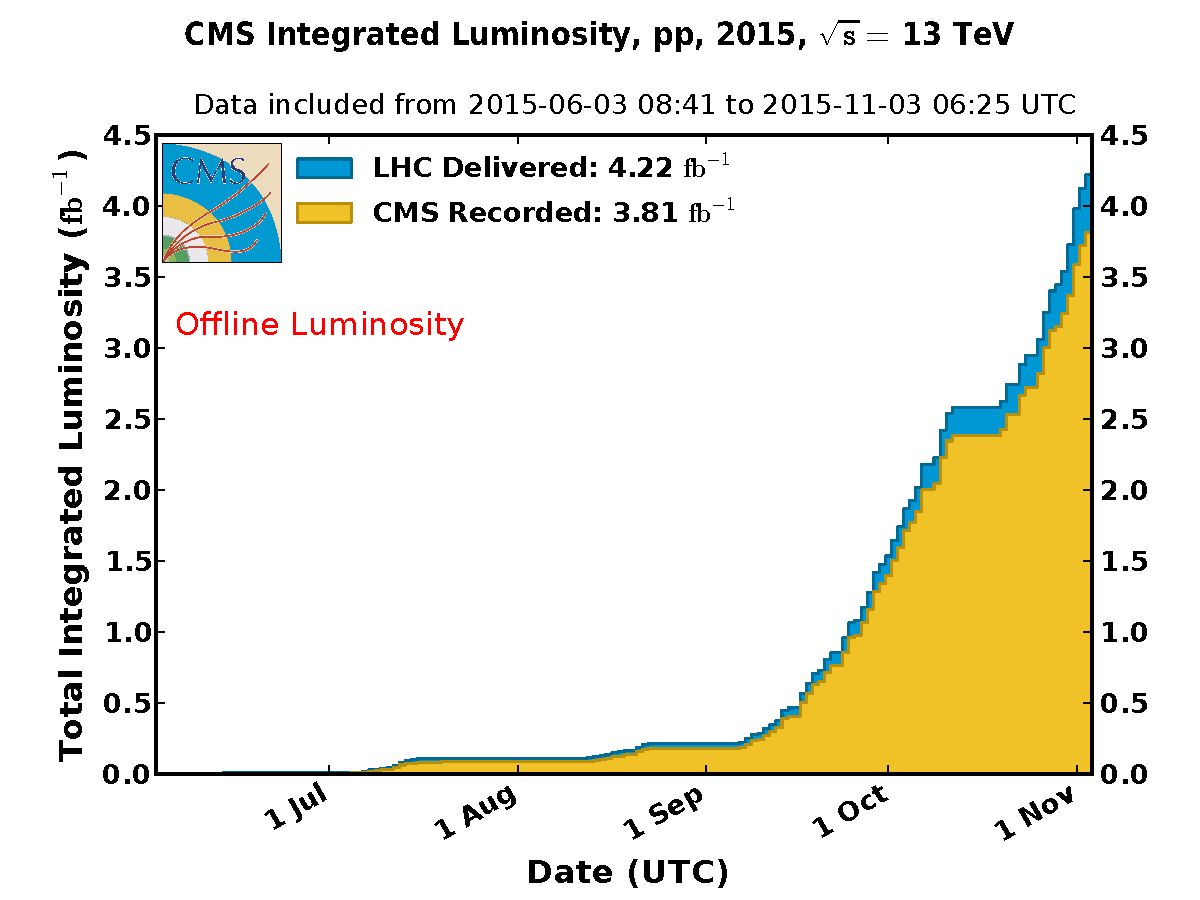
\includegraphics[width=1.0\textwidth]{figures/int_lumi_per_day_cumulative_pp_2015.pdf}
	\caption{Integrated luminosity delivered by the LHC, and recorded by CMS in 2015.}
	\label{fig:lhc2015IntegLumi}
\end{figure}


The raw dataset collected by CMS is too large ($\gtrsim 10^{4}$ terabytes) to process for analyses
which want to run from start to finish in $\lessim 3$ days, and contains much more information
than what is needed by any individual physics analysis.  To expedite the process of
transforming collision data into a public physics result, collision data from each run
era is split into several smaller datasets which are distinguished by the presence of one
or more objects in the final state, such as events with at least one muon, or least two
electrons or photons.  The HLT decides which dataset an event should be assigned to based on the
individual triggers which were fired; in some instances one event will be assigned to several
datasets.  As the average instantaneous luminosity of the LHC increased dramatically in the 
last 3 months of data-taking, datasets in Run2015D were split into two pieces such that the size
of each dataset remained small ($\sim 1$ terabyte).  The collision events used in this analysis
were collected in the "SingleMuon", "DoubleEG", and "MuonEG" datasets summarized in Table
\ref{tab:collisionDatasets}.  This analysis uses the datasets which were reconstructed, the process
by which raw detector outputs are transformed into distinguishable objects like muons and
electrons, in the late summer, fall and early winter of 2015 using calibration and alignment
constants derived in early 2015.

\begin{table}[h]
\caption{The collision datasets used in this analysis, the run eras they correspond to, and their total size (both dataset pieces for 2015D).}
\label{tab:collisionDatasets}
\centering
\begin{tabular}{c|c|c|c|c}
Run Era & Int. Lumi (pb$^{-1}$) & eejj dataset & $\mu\mu$jj dataset & e$\mu$jj dataset \\  \hline
	2015C &  20  &  DoubleEG  &  SingleMuon  &  MuonEG  \\
	2015D &  2620  &  DoubleEG  &  SingleMuon  &  MuonEG  \\ \hline
\end{tabular}
\end{table}

The "DoubleEG" dataset requires at least two energy deposits in ECAL 
consistent with electrons or photons.  The dataset is used to study events with two electrons and two jets
in the final state, and to look for evidence of \WR bosons which decay to electron flavor
heavy neutrinos.  During collisions, events are selected using the trigger $\verb|HLT_DoubleEle33_CaloIdL_GsfTrkIdVL|$.
As explained in Chapter \ref{sec:experiment_chapter}, the trigger first runs a subset of the full
particle reconstruction software package to reconstruct electron candidates in
every event.  After reconstruction, the trigger requires at least two electrons to pass
the cuts defined in Table \ref{tab:eleHltCuts}.  These cuts were optimized to increase the fraction
of real over fake electrons electrons selected by the trigger.
The ID variable cut thresholds differ between the ECAL barrel ($|\eta| \leq 1.42$)
and endcap ($|\eta| \geq 1.57$) for the following reason.  All ECAL crystals are used for event
triggering, but the way in which these crystals are grouped into trigger zones differs between the
barrel and endcap.  As a result, the shape and peak position of ID variables for real electrons
produced by $Z \rightarrow ee$ decays differs between barrel and endcap electrons.  The electron
ID variable cut thresholds differ between the barrel and endcap such that each ID cut selects
real barrel and endcap electrons with similar efficiencies.


\begin{table}[h]
\caption{Double electron trigger requirements.  The endcap $|\Delta\eta_{in}|$ or $|\Delta\sigma_{in}|$ cuts are
not applied as the endcap was not fully aligned with the tracker. NOT COMPLETE FINISH LATER}
\label{tab:eleHltCuts}
\centering
\begin{tabular}{c|c|c}
	Variable & Barrel cut threshold & Endcap cut threshold  \\  \hline
	energy and geometric acceptance cuts  &  &   \\
	$E_{T} (\GeV)$  &  33  &  33  \\
	$|\eta| (-)$  &  $< 2.5$  &  $< 2.5$  \\  \hline
	electron ID cuts  &  &  \\
	$\sigma_{i\eta i\eta} (-)$  &  $< 0.014$  &  $< 0.035$  \\
	$H/E (1/\GeV)$  &  $< 0.15/E_{T}$  &  $< 0.1/E_{T}$  \\
	ECAL Iso $(1/\GeV)$  &  $< EBISO/E_{T}$  &  $< EEISO/E_{T}$  \\
	HCAL Iso $(1/\GeV)$  &  $< HBISO/E_{T}$  &  $< HEISO/E_{T}$  \\
	$|\Delta\eta_{in}|$  &  $< 0.02$  &  $N/A$  \\
	$|\Delta\sigma_{in}|$  &  $< 0.15$  &  $N/A$  \\
	Tracker Iso $(1/\GeV)$  &  $< 0.125/p_{T}$  &  $< 0.125/p_{T}$  \\
\end{tabular}
\end{table}


This particular double electron trigger was chosen based on trigger efficiency, and offline (post trigger)
requirements which must be tighter than the trigger.  As shown in
Table \ref{tab:singleAndDblEleTriggers}, there is not a significant difference in trigger efficiency
between single and double electron triggers as long as single electron Level 1 triggers are utilized.
These efficiencies were calculated using events from the 800 $\GeV$ \WR mass $\WR \rightarrow eejj$
dataset, as events from this dataset have the lowest average leading and subleading electron $E_{T}$
of all $\WR \rightarrow eejj$ datasets considered in this search.  To ensure that most of offline (post trigger)
electron ID requirements are tighter than the electron trigger ID requirements, $\verb|HLT_DoubleEle33_CaloIdL_GsfTrkIdVL|$
was chosen over the higher $E_{T}$ and tighter ID single electron trigger.

\begin{table}[h]
\caption{Efficiency of electron triggers in 800 $\GeV$ \WR mass $\WR \rightarrow eejj$ signal events which have
two real, reconstructed electrons within the trigger acceptance ($|\eta| \leq 2.5$).  The double electron trigger
with lower $E_{T}$ cuts (23 and 12) can only fire if a double electron Level 1 trigger is fired, and thus has
a lower efficiency than the DoubleEle33 trigger which can fire if a double or single electron Level 1 trigger
is fired.}
\label{tab:singleAndDblEleTriggers}
\centering
\begin{tabular}{c|c|}
	Electron trigger & Efficiency (\%)  \\  \hline
	$\verb|HLT_Ele105_CaloIdVT_GsfTrkIdT|$  &  $94.8\pm0.2$  \\
	$\verb|HLT_DoubleEle33_CaloIdL_GsfTrkIdVL|$  &  $92.0\pm0.2$  \\
	$\verb|HLT_Ele23_Ele12_CaloIdL_TrackIdL_IsoVL|$  &  $91.0\pm0.2$  \\
\end{tabular}
\end{table}


The "SingleMuon" dataset requires at least one energy deposit in the muon detectors 
consistent with a muon.  This dataset is used to study events with two muons and two jets
in the final state, and to look for evidence of \WR bosons which decay to muon flavor
heavy neutrinos.  During collisions, events are selected using the trigger $\verb|HLT_Mu50|$.
The trigger first runs a subset of the full particle reconstruction software package to
reconstruct muon candidates in every event.  After reconstruction, the trigger requires at
least one muon candidate, made from a good quality track matched to a muon detector energy
deposit, to have $p_{T} > 50 \GeV$.

This particular single muon trigger was chosen based on trigger efficiency, and offline (post trigger)
requirements which must be tighter than the trigger.  As shown in
Table \ref{tab:singleAndDblMuTriggers}, there is not a significant difference in trigger efficiency
between single and double muon triggers as long as single muon Level 1 triggers are utilized.
Events from the 800 $\GeV$ \WR mass $\WR \rightarrow \mu\mu jj$ dataset have the lowest average
leading and subleading muon $p_{T}$ amongst all $\WR \rightarrow \mu\mu jj$ datasets used in this
analysis, so events from this dataset were used to determine the trigger efficiencies shown in
Table \ref{tab:singleAndDblMuTriggers}.  Ignoring prescaled triggers\footnote{there are triggers
which have lower $p_{T}$ thresholds than those listed here, but their rates are artificially
suppressed by randomly ignoring events which pass all trigger requirements} and triggers
which require tighter isolation requirements than the optimal offline muon isolation for this
search, the best trigger for this search is $\verb|HLT_Mu50|$.  Even though switching to lower $p_{T}$
threshold single and double muon triggers would allow for lower offline lepton $p_{T}$ cuts, it
will be shown later (see section \ref{muonRecoAndSelection}) that lower offline lepton cuts would reduce signal over background
sensitivity in the medium and high \WR mass region.


\begin{table}[h]
\caption{Efficiency of muon triggers in 800 $\GeV$ \WR mass $\WR \rightarrow \mu\mu jj$ signal events which have
two real, reconstructed muons within the trigger acceptance ($|\eta| \leq 2.4$).}
\label{tab:singleAndDblMuTriggers}
\centering
\begin{tabular}{c|c|}
	Muon trigger & Efficiency (\%)  \\  \hline
	$\verb|HLT_Mu50|$  &  $98.4\pm0.1$  \\
	$\verb|HLT_Mu45_eta2p1|$  &  $97.6\pm0.1$  \\
	$\verb|HLT_Mu40_TkMu11|$  &  $96.9\pm0.1$  \\
	$\verb|HLT_Mu34|$  &  $99.1\pm0.1$  \\
\end{tabular}
\end{table}


The "MuonEG" dataset requires at least one energy deposit in the muon detectors consistent
with a muon, and at least one energy deposit in ECAL consistent with an electron or photon.
This dataset is used to study events with one electron, one muon and two jets
in the final state.  We seek a \WR boson whose decay conserves lepton flavor, so to leading
order in the right handed electroweak coupling there cannot be any excess of events in the
$e\mu jj$ final state due to a \WR boson.  Thus, the $e\mu jj$ final state is only used to estimate
backgrounds from the top quark.  During collisions, events are selected using the trigger
$\verb|HLT_Mu30_Ele30_CaloIdL_GsfTrkIdVL|$.  The trigger first runs a subset of the full
particle reconstruction software package to reconstruct muon and electron candidates in
every event.  After reconstruction, the trigger requires at least one muon candidate, made
from a good quality track geometrically matched to a muon detector energy deposit, to have
$p_{T} > 30 \GeV$.  In addition, at least one electron candidate which passes loose ID cuts
must be found with $E_{T} > 30 \GeV$.  As this trigger is only used for background estimation
in the signal region, it was chosen because it replicates the trigger algorithms and
lepton ID cut thresholds used to select $\mu\mu jj$ events from the "SingleMuon" dataset, and eejj events
from the "DoubleEG" dataset, but uses lower $E_{T}$ and $p_{T}$ cuts.

In addition to the trigger requirements discussed above, collision datasets are cleaned of events
in which global reconstruction problems occurred within the detector.  These include events
where no primary vertex is reconstructed, and when anomalous noise appears in the
tracker, calorimeters, or muon detectors.  Furthermore, events identified as coming from
interactions between a single proton beam and beam pipe gas or other foreign material are
removed.


\subsection{Monte Carlo}
\label{MC}
Monte Carlo (\MC) simulations were used to estimate backgrounds and systematic uncertainties, derive
scale factors, reinterpret \WR cross section limits, and identify kinematic regions for
hypothetical \WR boson signals with specific \WR masses.  The \MC samples used to estimate backgrounds
and systematic uncertainties, identify kinematic regions for specific \WR boson signals, and derive
scale factors were produced by the CMS \MC production group.  Events produced by this group were
passed through a full simulation of the CMS detector using GEANT4 \cite{geant4}, were hadronized\footnote{hadronization
is the process through which unstable quarks and gluons produced at the Feynman diagram level of simulation
are transformed into stable jets observed by CMS} using \PYTHIA, and detector information was reconstructed
into particles using the same CMS particle reconstruction library used with collision data.
Fully reconstructed simulated events were required to pass the same trigger as the collision
data events they were being compared to.  For example, \DY +jet events used to estimate the SM
background in the eejj ($\mu\mu jj$) final state were required to pass the double electron
(single muon) trigger discussed earlier (section \ref{dataAndTriggers}).
\MC samples were produced by the CMS \MC production group for all SM processes which can yield
the same final state as a \WR boson at an appreciable rate\footnote{for example, Vector Boson Fusion production
of diboson pairs is not considered due to its low cross section times branching
fraction}, and high cross section SM processes which can produce two jets
and two fake leptons.  These processes are \DY (DY)+jets, W+jets, t$\bar{t}$+jets generated
with \MADGRAPH \cite{madgraph}, single top and top+W generated with \POWHEG \cite{powheg}, and
QCD and diboson (WW, WZ, ZZ) generated with \PYTHIA \cite{pythia8}\cite{Sjostrand:2006za}.
These samples and their generators are listed in Table \ref{tab:centrallyProducedMC} along
with their cross sections, and the number of events in each sample.

\begin{table}[bt]
\caption{Fully reconstructed \MC samples produced by the CMS \MC production group.  Cross sections
	are calculated at next-to-leading order (NLO) unless noted otherwise.  The \DY and t$\bar{t}$+jets events
were produced with a dilepton mass $M_{LL} > 50 \GeV$ cut using the two
leptons coming from the hard interaction.}
\label{tab:centrallyProducedMC}

\centering
\resizebox{\textwidth}{!}{
	\begin{tabular}{ |c|c|c|c| } 
	\hline
		Dataset         & Generator & $\sigma$ $\times$ filter efficiency (pb) & Events   \\
		\hline
		Inclusive DY+jets, $DY \rightarrow ll$ & \MADGRAPH   & 5991 (LO)   & 9042031 \\ \hline
		DY+jets HT 100-200, $DY \rightarrow ll$ & \MADGRAPH   & 181.3 (LO)   & 2725655 \\ \hline
		DY+jets HT 200-400, $DY \rightarrow ll$ & \MADGRAPH   & 50.42 (LO)   & 973937 \\ \hline
		DY+jets HT 400-600, $DY \rightarrow ll$ & \MADGRAPH   & 6.984 (LO)   & 1067758 \\ \hline
		DY+jets HT $>$ 600, $DY \rightarrow ll$ & \MADGRAPH   & 2.704 (LO)   & 998912 \\ \hline
		\ttbar+jets $\rightarrow ll$+jets & \MADGRAPH  & 85.67 (LO)   & 24521141 \\ \hline
		single t $\rightarrow$ leptons+jets  & \POWHEG & 80.95 & 1680200 \\ \hline
		single $\bar{t}$ $\rightarrow$ leptons+jets & \POWHEG & 136.0 & 3299800 \\ \hline
		$\bar{t}$+W   & \POWHEG & 35.85 & 988500 \\ \hline
		t+W   & \POWHEG & 35.85 & 995600 \\ \hline
		WW  & \PYTHIA & 113.8   & 993640   \\ \hline
		ZZ  & \PYTHIA & 10.15   & 996944   \\ \hline
		WZ  & \PYTHIA & 23.4   & 978512   \\ \hline
		W+jets, $W \rightarrow l\nu$ & \MADGRAPH & 50270 (NNLO)   & 72207128 \\ \hline
		QCD Pt 15-20 $e\gamma$ enriched  & \PYTHIA & 2302200   & 2122959   \\ \hline
		QCD Pt 15-20 $\mu$ enriched  & \PYTHIA & 3819570   & 2362016   \\ \hline
		QCD Pt 20-30 $e\gamma$ enriched  & \PYTHIA & 5352960     & 9184197   \\ \hline
		QCD Pt 20-30 $\mu$ enriched  & \PYTHIA & 2960198    & 5311955   \\ \hline
		QCD Pt 30-50 $e\gamma$ enriched  & \PYTHIA & 9928000    & 4736965   \\ \hline
		QCD Pt 30-50 $\mu$ enriched  & \PYTHIA & 1652471    & 4946084   \\ \hline
		QCD Pt 50-80 $e\gamma$ enriched  & \PYTHIA & 2890800    & 5291543   \\ \hline
		QCD Pt 50-80 $\mu$ enriched  & \PYTHIA & 437504     & 5058536   \\ \hline
		QCD Pt 80-120 $e\gamma$ enriched  & \PYTHIA & 350000  & 8130424   \\ \hline
		QCD Pt 80-120 $\mu$ enriched  & \PYTHIA & 106034    & 3882463   \\ \hline
		QCD Pt 120-170 $e\gamma$ enriched  & \PYTHIA & 62964   & 8513976   \\ \hline
		QCD Pt 120-170 $\mu$ enriched  & \PYTHIA & 25191    & 4026104   \\ \hline
		QCD Pt 170-300 $\mu$ enriched  & \PYTHIA & 8654     & 3949716   \\ \hline
		QCD Pt 170-300 $e\gamma$ enriched  & \PYTHIA & 18810     & 5735584   \\ \hline
		QCD Pt $>$ 300 $e\gamma$ enriched  & \PYTHIA & 1350    & 3707833   \\ \hline
		QCD Pt 300-470 $\mu$ enriched  & \PYTHIA & 797.4     & 3960205   \\ \hline
		QCD Pt 470-600 $\mu$ enriched  & \PYTHIA & 79.03     & 1928595   \\ \hline
		QCD Pt 600-800 $\mu$ enriched  & \PYTHIA & 25.1      & 1983363   \\ \hline
		QCD Pt 800-1000 $\mu$ enriched  & \PYTHIA & 4.71     & 1982314   \\ \hline
		QCD Pt $>$ 1000 $\mu$ enriched  & \PYTHIA & 1.62      & 1981954   \\ \hline
		$\WR \rightarrow l\Nell$  & \PYTHIA & 1$\times 10^{-5}$ - 4.3 & 50000   \\ \hline
		\end{tabular}
}
\end{table}

The CMS \MC production group also generated \WR signal samples, with both eejj and $\mu\mu jj$
final states, using the Left-Right Symmetric SM extension model built into \PYTHIA.  Specific
features of this model are explained in section \ref{sec:theory_chapter}.  \WR signal
samples were produced with $M_{\Nell} = M_{\WR}/2$, and $M_{\WR}$ starting at 800 $\GeV$ and
increasing, in increments of 200 $\GeV$, to 6000 $\GeV$.  The electron and muon triggers
discussed earlier must also be fired in these \WR signal events.

The number of reconstructed interaction vertices from all collision datasets described
earlier approximates a Poisson distribution, and the average number of reconstructed
interaction vertices in each event in 2015 was above 9.  In each collision event, this
set of interaction vertices is comprised of the primary interaction vertex which
resulted in one or more lepton triggers firing, and secondary interaction vertices,
typically caused by QCD, which resulted in additional energy being measured by CMS.
These secondary interaction vertices are created as a result of the high instantaneous
luminosity, and, in the context of this search, their only effect is to obfuscate
signs of a \WR boson.  To reproduce the effect of secondary interaction vertices, all
simulated event samples produced by the CMS \MC group are mixed with "minimum bias"
events before simulating the detector response and subsequent particle reconstruction.
Each minimum bias event has only one interaction vertex that results in at least
one particle travelling into CMS with sufficient energy to be detected\footnote{The minimum
bias events mixed into simulated events, in principle, can come from any known and
well measured SM process.  However, the enormous cross section of proton proton
inelastic scattering and other low momentum transfer QCD processes means the vast
majority of minimum bias events come from low momentum transfer QCD processes}.
The number of minimum bias events mixed into one simulated event is determined
by sampling a random number from a Poisson distribution whose mean was set equal
to the expected number of average reconstructed vertices in 2015 collision events.
This expected average was calculated before 2015 collisions began, so \MC events 
used in this analysis are reweighted based on the true difference between reconstructed
vertices in \MC and collision data.

A set of \WR \MC signal samples were privately produced only to extend \WR cross
section limits set for $M_{\Nell} = M_{\WR}/2$ to a 2D plane of possible \WR
and \Nell mass values.  These private samples were produced using the same
\PYTHIA generator and parameters used by the CMS \MC production group, but the
detector response simulation and particle reconstruction steps were omitted.
In addition, no trigger requirements are applied.
Samples were produced starting at $M_{\WR} = 800 \GeV$
and $M_{\Nell} = 100 \GeV$, and $M_{\WR}$ increasing to 4000 $\GeV$ in increments
of 100 $\GeV$.  At each $M_{\WR}$, 15000 events are produced for every $M_{\Nell}$
value, starting at 100 $\GeV$ and increasing in increments of 100 $\GeV$ up to
$M_{\Nell} = M_{\WR} - 100 \GeV$.


\section{Jet and Lepton Reconstruction and Selection}

\subsection{Jet Reconstruction and Selection}
\label{jetRecoAndSelection}
The Particle Flow (PF) algorithm, introduced in Chapter \ref{sec:experiment_chapter}, is used
to reconstruct all particles which interact with the tracker, calorimeters and muon
detectors of CMS.  Reconstructed particles are grouped into five categories, each with their
own distinguishing features, shown in Table \ref{tab:pfRecoBins}.  Information
from every subdetector is combined to determine the energy and momentum of
each reconstructed particle.  Jets originate from unstable quarks and gluons,
but what is actually detected are the stable daughter particles created by
quark and gluon decays.  These include stable charged and neutral hadrons ($\pi^{\pm}$,
$K^{0}$), stable charged leptons ($e^{\pm}$, $\mu^{\pm}$) created by weak boson
decays, and photons resulting from electromagnetic decays of neutral hadrons like
the $\pi^{0}$.  Thus, all particles reconstructed by the PF algorithm are considered
during jet reconstruction.

\begin{table}[h]
\caption{The Particle Flow algorithm reconstructs particles, and, based on the reconstructed
track and or calorimeter information, assigns each particle to one of these categories.}
\label{tab:pfRecoBins}
\centering
\begin{tabular}{c|c}
Particle Category & Distinguishing Features \\  \hline
	Photon &  has no track, only energy in ECAL  \\ \hline
	Electron &  has track geometrically linked to energy in ECAL  \\ \hline
	Muon &  has track geometrically linked to energy in muon detector  \\ \hline
	Charged Hadron &  has track geometrically linked to energy in HCAL or HCAL and ECAL  \\ \hline
	Neutral Hadron &  has no track, only energy in HCAL or HCAL and ECAL  \\ \hline
\end{tabular}
\end{table}

In each event the vertex with the highest $\Sigma p_{T}$ of all tracks is identified
as the primary vertex, and all other reconstructed vertices are pileup
vertices.
Charged hadrons, electrons and muons whose tracks come from pileup vertices
are removed from the list of possible jet constituents to mitigate the effect
of pileup interactions.  The remaining reconstructed particles are clustered
into jets using the anti-$k_{T}$ algorithm \cite{antikt}.  This algorithm
takes the $i^{th}$ particle from the list of possible jet constituents, and
calculates the distance parameter $d_{ij}$

\begin{equation}
	$d_{ij} = min(k_{Ti}^{-2},k_{Tj}^{-2})\frac{\Delta^{2}}{R^{2}}$
\end{equation}

using the $j^{th}$ particle in the same list, where $\Delta$ is the angular
separation between the $i^{th}$ and $j^{th}$ particle, R is 0.4, and $k_{Ti}$
is the $p_{T}$ of the $i^{th}$ particle.  If the $i^{th}$ particle has 
$d_{ij} > k_{Ti}^{-2}$ for all j, then the $i^{th}$ particle is a jet constituent
and is removed from the constituent list and placed in a new list $L_{1}$.
This procedure is repeated for all particles in the list of possible jet constituents,
then repeated for all elements in the new list $L_{1}$.  The iteration over
all particles in the newly created list continues N times, creating N lists,
until the lists $L_{N}$ and $L_{N-1}$ have the same number of elements.

Once the jets are clustered, their raw energies ($ = \Sigma E$ of constituents)
are corrected in several steps.  Neutral hadrons produced by pileup interactions
can still be clustered into jets, so the first correction reduces the energy
of every jet in a data or simulated event based on the jet area and the total neutral hadron
energy density in the event \cite{pileup1} \cite{pileup2}.  Subsequently, energy corrections based on jet $\eta$
and $p_{T}$ are applied.  These corrections, derived from \MC and applied to
jets in data and simulated events, brings the reconstructed jet $p_{T}$ into closer
agreement with the true (quark-gluon level) jet $p_{T}$ across the entire
range of reconstructed jet $p_{T}$ and $\eta$.  A second set of $p_{T}$ and
$\eta$ dependent energy corrections, derived from \MC and applied to data
events, bring the jet response in data into closer agreement with the jet
response in \MC.  More details on jet energy corrections, such as the types
of \MC events used to derive the corrections, can be found elsewhere \cite{jetpaper}.

After jets in data and simulation are reconstructed and corrected, jet
identification, acceptance and energy requirements are applied.  The
identification and acceptance criteria require each jet to have

\begin{itemize}
	\item $|\eta| \leq 2.4$
	\item less than 90\% of its energy comes from neutral hadrons
	\item less than 90\% of its energy comes from photons
	\item at least 2 constituents (from reconstructed PF particles)
	\item more than 0\% of its energy comes from charged hadrons
	\item at least one constituent is a charged hadron
	\item less than 99\% of its energy comes from electrons
\end{itemize}

The identification requirements are designed to increase the fraction of
selected jets which originate from real hadronic activity.  After acceptance
and identification cuts, all jets must have $p_{T} > 40 \GeV$.  Lowering
the jet $p_{T}$ cut was explored, as a lower cut would increase sensitivity
to \WR signals with \WR mass below 1.8 $\TeV$.  However, as shown in Table
\ref{tab:lowerJetPtCuts}, a lower $p_{T}$ cut on the subleading jet would
increase backgrounds without a corresponding increase in \WR signal.

\begin{table}[h]
	\caption{Signal/$\sqrt{Background}$ (S/$\sqrt{B}$) for subleading jet $p_{T}$
		cuts using simulated \DY, t$\bar{t}$ and $\WR \rightarrow \mu\mu jj$ events
	with $\mWR = 2.2 \TeV$ and $\mnuR = 1.1 \TeV$.  Lowering the cut would worsen S/$\sqrt{B}$.}
	\label{tab:lowerJetPtCuts}
	\centering
	\begin{tabular}{c|c}
		Sublead jet $p_{T}$ cut (\GeV) & S/$\sqrt{B}$ \\  \hline
		30 &  12.1  \\ \hline
		40 &  12.6  \\ \hline
	\end{tabular}
\end{table}

\subsection{Muon Reconstruction and Selection}
\label{muonRecoAndSelection}
The search for \WR signals in events with two final state $\mu$s .

%The PF algorithm reconstructs tracks from charged particles, and electromagnetic energy
%clusters from ECAL energy deposits.  Each electron candidate is then built from a track
%whose end point and trajectory are geometrically matched to at least one ECAL energy
%cluster.  If several real electrons (or positrons) have well separated tracks that point
%towards the same ECAL energy cluster, then that ECAL cluster will be shared between
%several PF electron candidates.
%
%After reconstruction, electron candidates are .
%
%Once the jets are clustered, their raw energies ($ = \Sigma E$ of constituents)
%are corrected in several steps.  Neutral hadrons produced by pileup interactions
%can still be clustered into jets, so the first correction reduces the energy
%of every jet in a data or simulated event based on the jet area and the total neutral hadron
%energy density in the event \cite{pileup1} \cite{pileup2}.  Subsequently, energy corrections based on jet $\eta$
%and $p_{T}$ are applied.  These corrections, derived from \MC and applied to
%jets in data and simulated events, brings the reconstructed jet $p_{T}$ into closer
%agreement with the true (quark-gluon level) jet $p_{T}$ across the entire
%range of reconstructed jet $p_{T}$ and $\eta$.  A second set of $p_{T}$ and
%$\eta$ dependent energy corrections, derived from \MC and applied to data
%events, bring the jet response in data into closer agreement with the jet
%response in \MC.  More details on jet energy corrections, such as the types
%of \MC events used to derive the corrections, can be found elsewhere \cite{jetpaper}.
%
%After jets in data and simulation are reconstructed and corrected, jet
%identification, acceptance and energy requirements are applied.  The
%identification and acceptance criteria require each jet to have
%
%\begin{itemize}
%	\item $|\eta| \leq 2.4$
%	\item less than 90\% of its energy comes from neutral hadrons
%	\item less than 90\% of its energy comes from photons
%	\item at least 2 constituents (from reconstructed PF particles)
%	\item more than 0\% of its energy comes from charged hadrons
%	\item at least one constituent is a charged hadron
%	\item less than 99\% of its energy comes from electrons
%\end{itemize}
%
%The identification requirements are designed to increase the fraction of
%selected electrons which originate from real electromagnetic activity.  After acceptance
%and identification cuts, all jets must have $p_{T} > 40 \GeV$.  Lowering
%the jet $p_{T}$ cut was explored, as a lower cut would increase sensitivity
%to \WR signals with \WR mass below 1.8 $\TeV$.  However, as shown in Table
%\ref{tab:lowerMuonPtCuts}, a lower $p_{T}$ cut on the subleading jet would
%increase backgrounds without a corresponding increase in \WR signal.
%
%\begin{table}[h]
%	\caption{Signal/$\sqrt{Background}$ (S/$\sqrt{B}$) for $\mu$ $p_{T}$
%		cuts using simulated \DY, t$\bar{t}$ and $\WR \rightarrow \mu\mu jj$ events
%	with $\mWR = 2.2 \TeV$ and $\mnuR = 1.1 \TeV$.  Lowering these cuts would worsen S/$\sqrt{B}$.}
%	\label{tab:lowerMuonPtCuts}
%	\centering
%	\begin{tabular}{c|c|c}
%		final state particle & $p_{T}$ cut (\GeV) & S/$\sqrt{B}$ \\  \hline
%		sublead $\mu$ & 40 &  11.9  \\
%		sublead $\mu$ & 53 &  12.6  \\ \hline
%		lead $\mu$ & 50 &  12.1  \\
%		lead $\mu$ & 60 &  12.6  \\ \hline
%	\end{tabular}
%\end{table}



\subsection{Electron Reconstruction and Selection}
\label{eleRecoAndSelection}
The PF algorithm reconstructs tracks from charged particles, and electromagnetic energy
clusters from ECAL energy deposits.  Each electron candidate is then built from a track
whose end point and trajectory are geometrically matched to at least one ECAL energy
cluster.  If several real electrons (or positrons) have well separated tracks that point
towards the same ECAL energy cluster, then that ECAL cluster will be shared between
several PF electron candidates.

%After reconstruction, electron candidates are .
%
%Once the jets are clustered, their raw energies ($ = \Sigma E$ of constituents)
%are corrected in several steps.  Neutral hadrons produced by pileup interactions
%can still be clustered into jets, so the first correction reduces the energy
%of every jet in a data or simulated event based on the jet area and the total neutral hadron
%energy density in the event \cite{pileup1} \cite{pileup2}.  Subsequently, energy corrections based on jet $\eta$
%and $p_{T}$ are applied.  These corrections, derived from \MC and applied to
%jets in data and simulated events, brings the reconstructed jet $p_{T}$ into closer
%agreement with the true (quark-gluon level) jet $p_{T}$ across the entire
%range of reconstructed jet $p_{T}$ and $\eta$.  A second set of $p_{T}$ and
%$\eta$ dependent energy corrections, derived from \MC and applied to data
%events, bring the jet response in data into closer agreement with the jet
%response in \MC.  More details on jet energy corrections, such as the types
%of \MC events used to derive the corrections, can be found elsewhere \cite{jetpaper}.
%
%After jets in data and simulation are reconstructed and corrected, jet
%identification, acceptance and energy requirements are applied.  The
%identification and acceptance criteria require each jet to have
%
%\begin{itemize}
%	\item $|\eta| \leq 2.4$
%	\item less than 90\% of its energy comes from neutral hadrons
%	\item less than 90\% of its energy comes from photons
%	\item at least 2 constituents (from reconstructed PF particles)
%	\item more than 0\% of its energy comes from charged hadrons
%	\item at least one constituent is a charged hadron
%	\item less than 99\% of its energy comes from electrons
%\end{itemize}
%
%The identification requirements are designed to increase the fraction of
%selected electrons which originate from real electromagnetic activity.  After acceptance
%and identification cuts, all jets must have $p_{T} > 40 \GeV$.  Lowering
%the jet $p_{T}$ cut was explored, as a lower cut would increase sensitivity
%to \WR signals with \WR mass below 1.8 $\TeV$.  However, as shown in Table
%\ref{tab:lowerJetPtCuts}, a lower $p_{T}$ cut on the subleading jet would
%increase backgrounds without a corresponding increase in \WR signal.
%
%\begin{table}[h]
%	\caption{Signal/$\sqrt{Background}$ (S/$\sqrt{B}$) for subleading jet $p_{T}$
%		cuts using simulated \DY, t$\bar{t}$ and $\WR \rightarrow \mu\mu jj$ events
%	with $\mWR = 2.2 \TeV$ and $\mnuR = 1.1 \TeV$.  Lowering the cut would worsen S/$\sqrt{B}$.}
%	\label{tab:lowerElePtCuts}
%	\centering
%	\begin{tabular}{c|c}
%		Sublead jet $p_{T}$ cut (\GeV) & S/$\sqrt{B}$ \\  \hline
%		30 &  12.1  \\ \hline
%		40 &  12.6  \\ \hline
%	\end{tabular}
%\end{table}



%%%%%%%%%%%%%%%%%%%%%%%%%%%%%%%%%%%%%%%%%%%%%%%%%%%%%%%%%%%%%%%%%%%%%%%%%%%%%%%%
